% --- Template for thesis / report with tktltiki2 class ---
% 
% last updated 2013/02/15 for tkltiki2 v1.02

\documentclass[finnish]{tktltiki2}

% tktltiki2 automatically loads babel, so you can simply
% give the language parameter (e.g. finnish, swedish, english, british) as
% a parameter for the class: \documentclass[finnish]{tktltiki2}.
% The information on title and abstract is generated automatically depending on
% the language, see below if you need to change any of these manually.
% 
% Class options:
% - grading                 -- Print labels for grading information on the front page.
% - disablelastpagecounter  -- Disables the automatic generation of page number information
%                              in the abstract. See also \numberofpagesinformation{} command below.
%
% The class also respects the following options of article class:
%   10pt, 11pt, 12pt, final, draft, oneside, twoside,
%   openright, openany, onecolumn, twocolumn, leqno, fleqn
%
% The default font size is 11pt. The paper size used is A4, other sizes are not supported.
%
% rubber: module pdftex

% --- General packages ---

\usepackage[utf8]{inputenc}
\usepackage[T1]{fontenc}
\usepackage{lmodern}
\usepackage{microtype}
\usepackage{amsfonts,amsmath,amssymb,amsthm,booktabs,color,enumitem,graphicx}
\usepackage[pdftex,hidelinks]{hyperref}
\usepackage{listings}
\usepackage{xcolor}
\usepackage{amsmath}
\usepackage{graphicx}
\lstset{
	keywordstyle=\color{black}\bfseries, % style for keywords
	numbers=none, % where to put the line-numbers
	numberstyle=\tiny, % the size of the fonts that are used for the line-numbers     
	showspaces=false, % shcow spaces adding particular underscores
	showstringspaces=false, % underline spaces within strings
	showtabs=false, % show tabs within strings adding particular underscores
	frame=single, % adds a frame around the code
	framesep=5pt,
	aboveskip=15pt,
	belowskip=15pt,
	tabsize=2, % sets default tabsize to 2 spaces
	rulesepcolor=\color{gray},
	rulecolor=\color{black},
	captionpos=b, % sets the caption-position to bottom
	breaklines=true, % sets automatic line breaking
	breakatwhitespace=false,
	literate={ö}{{\"o}}1
	{ä}{{\"a}}1
	{ü}{{\"u}}1
}

% Automatically set the PDF metadata fields
\makeatletter
\AtBeginDocument{\hypersetup{pdftitle = {\@title}, pdfauthor = {\@author}}}
\makeatother

% --- Language-related settings ---
%
% these should be modified according to your language

% babelbib for non-english bibliography using bibtex
\usepackage[fixlanguage]{babelbib}
\selectbiblanguage{finnish}

% add bibliography to the table of contents
\usepackage[nottoc]{tocbibind}
% tocbibind renames the bibliography, use the following to change it back
\settocbibname{Lähteet}

% --- Theorem environment definitions ---

\newtheorem{lau}{Lause}
\newtheorem{lem}[lau]{Lemma}
\newtheorem{kor}[lau]{Korollaari}

\theoremstyle{definition}
\newtheorem{maar}[lau]{Määritelmä}
\newtheorem{ong}{Ongelma}
\newtheorem{alg}[lau]{Algoritmi}
\newtheorem{esim}[lau]{Esimerkki}

\theoremstyle{remark}
\newtheorem*{huom}{Huomautus}


% --- tktltiki2 options ---
%
% The following commands define the information used to generate title and
% abstract pages. The following entries should be always specified:

\title{SQL-Injektio ja siltä suojautuminen}
\author{Lalli Nuorteva}
\date{\today}
\level{Kandidaatintutkielma}
\abstract{Tiivistelmä.}

% The following can be used to specify keywords and classification of the paper:

\keywords{avainsana 1, avainsana 2, avainsana 3}

% classification according to ACM Computing Classification System (http://www.acm.org/about/class/)
% This is probably mostly relevant for computer scientists
% uncomment the following; contents of \classification will be printed under the abstract with a title
% "ACM Computing Classification System (CCS):"
% \classification{}

% If the automatic page number counting is not working as desired in your case,
% uncomment the following to manually set the number of pages displayed in the abstract page:
%
% \numberofpagesinformation{16 sivua + 10 sivua liitteissä}
%
% If you are not a computer scientist, you will want to uncomment the following by hand and specify
% your department, faculty and subject by hand:
%
% \faculty{Matemaattis-luonnontieteellinen}
% \department{Tietojenkäsittelytieteen laitos}
% \subject{Tietojenkäsittelytiede}
%
% If you are not from the University of Helsinki, then you will most likely want to set these also:
%
% \university{Helsingin Yliopisto}
% \universitylong{HELSINGIN YLIOPISTO --- HELSINGFORS UNIVERSITET --- UNIVERSITY OF HELSINKI} % displayed on the top of the abstract page
% \city{Helsinki}
%


\begin{document}
	
	% --- Front matter ---
	\frontmatter      % roman page numbering for front matter
	
	\maketitle        % title page
	%\makeabstract     % abstract page
	
	\tableofcontents  % table of contents
	
	% --- Main matter ---
	
	\mainmatter       % clear page, start arabic page numbering
	
	\section{Johdanto}
	Tämän kandidaatintutkielman päätavoite on selvittää kuinka SQL-injektiolta voidaan suojautua mahdollisimman tehokkaasti. Tutkielmassa esitellään ensiksi mikä on SQL-injektio. Esittelyssä paneudutaan siihen miten SQL-injektio voidaan toteuttaa käytännössä, sekä millaisiin eri alatyyppeihin SQL-injektiot voidaan jaotella. Tämän jälkeen esitellään erilaisia tapoja suojautua SQL-injektioilta. Suojautumistavat on jaettu kolmeen eri osa-alueeseen: ohjelmointikäytänteet, ajonaikainen monitorointi ja sovelluksen testaaminen. Hyvien ohjelmointikäytänteiden ja ajonaikaisen monitoroinnin avulla pyritään toteuttamaan sovellus johon SQL-injektiot eivät ole mahdollisia. Jotta tavoitteen suojautumisen onnistumisesta voitaisiin olla varmoja, tulee sovellusta testata. Tutkielman testausosiossa esitellään automatisoituja tapoja toteuttaa sovelluksen testaaminen.
	
	Tutkimusten mukaan 8\% web-palveluista sisältää haavoittuvaisuuksia.  87\% Näistä haavoittuvuuksista on SQL-injektio haavoittuvuuksia \cite{detection}. Yleisyytensä lisäksi SQL-injektio on myös hyvin vaarallinen. Onnistuneen SQL-injektion avulla hyökkääjä voi suorittaa huonosti suojatussa tietokannassa mitä tahansa operaatioita. Tämä mahdollistaa esimerkiksi arkuluontoisten tietojen lukemisen ja muokkaamisen, tai esimerkiksi sovelluksen autentikaation ohittamisen. SQL-Injektiolla on vuosien aikana tehty lukuisia murtoja. SQL-Injektio mielletään monesti amatöörien ongelmaksi, mutta  sen avulla on murretty myös paljon ammattilaisten ohjelmoimia järjestelmiä. Yksi suurimmista SQL-Injektion avulla tehdyistä murroista tehtiin Guess.com:ille. Hyökkääjä sai käsinsä 200 000 ihmisen nimet ja luottokorttitiedot.
	
	Sen lisäksi että SQL-injektio on yleisin tietoturva-aukko, se on myös helppoa toteuttaa ilman syvällistä ymmärrystä sen toiminnasta. Esimerkiksi penetraatiotestaus \textit{(engl. penetration testing)} työkalut, kuten "sqlmap"\space, ilmoittavat sivuston heikkouksita melkeinpä napin painalluksella. Vaikka sqlmapin kaltaiset työkalut onkin tehty nimenomaan penetraatiotestaukseen, mikään ei estä hyökkääjää käyttämästä sitä apuna.
	
	Erilaisten palveluiden siirtyessä verkkoon, verkossa käsitellään jatkuvasti entistä enemmän arkaluontoisia tietoja. Verkossa hoidetaan asioita kuten laskujen maksaminen, hotellien varaus ja henkilökohtaisten viestien vaihtaminen. Yleensä tiedot tallennetaan relaatiotietokantoihin. Juuri tällaiset sovellukset voivat olla haavoittuvaisia SQL-Injektioille, ellei siltä olla suojauduttu oikeaoppisesti. Tästä syystä jokaisen tietokantasovelluksia ohjelmoivan on ymmärettävä mikä on SQL-injektio ja kuinka suojautua siltä voidaan suojautua.
	

	
	
	
	\section{SQL-Injektio}
	
	Anleyn artikkelin "Advancen SQL Injections in SQL Server Applications"\space mukaan SQL-Injektio hyökkäys esiintyy sillon, kun hyökkääjä pääsee muuttamaan SQL käskyn logiikkaa, semantiikkaa tai syntaksia. Tämä tapahtuu lisäämällä alkuperäiseen kyselyyn uusia SQL avainsanoja tai operaattoreita.
	Mikäli sovelluksen tietokantaoikeuksia ei ole erikseen rajattu, hyökkääjä voi onnistuneen SQL-injektion seurauksena suorittaa mitä tahansa tietokantapalvelimen tukemia SQL-kyselyitä. Jotkut tietokantapalvelimet sallivat myös käyttöjärjestelmätason komentojen suorittamisen. Tällöin hyökkääjän on mahdollista suorittaa myös muunlaisia hyökkäyksiä. 
	
	SQL-Injektio on mahdollinen vain silloin kun käyttäjältä tulevaa tietoa käytetään osana tietokantapalvelimelle tehtävää kyselyä. Tämä on kuitenkin varsin tavallinen tarve sovelluksissa. Tietokannassa voidaan säilyttää esimerkiksi käyttäjätunnuksia ja salasanoja. Näin ollen kirjautuessa järjestelmään käyttäjän antamaa syötettä käytetään osana SQL-kyselyä.
	
	\subsection{SQL-Injektio käytännössä}
	
 Esimerkiksi tuotteiden etsimiseen liittyvä SQL-käsky voidaan rakentaa huonosti suunitellussa sovelluksessa seuraavalla tavalla:
 
	\begin{lstlisting}
	sql = "SELECT * FROM tuotteet
	WHERE nimi ='" + params[:tuotenimi]
	\end{lstlisting}
	
	Mikäli käyttäjä antaa nimekseen "'; DROP TABLE tuottet'. Valmis kysely tietokannalle näyttää seuraavalta:
	
	\begin{lstlisting}[language=sql]
	sql = "SELECT * FROM tuotteet
	WHERE nimi =''; DROP TABLE tuotteet     
	\end{lstlisting}
	
	Kyseinen kysely etsii ensin kaikki tuotteet joiden nimi on tyhjä. Seuraavaksi suoritetaan komento "DROP TABLE tuotteet", joka poistaa koko tuotteet taulun.
	
	"DROP TABLE tuotteet"\space tilalla olisi voinut olla mikä tahansa muukin SQL-kysely. Esimerkiksi kaikkien tuotteiden listaamiseen hyökkääjä olisi voinut käyttää tuotenimeä joka sisältää jonkin tautologian esimerkiksi "'; OR 1=1". Liittääkseen vastaukseen jonkin muun taulun hyökkääjä olisi voinut käyttää UNION:ia.
	
	\subsubsection{Obfuskointi}
	
	Salgadon kirjoittaman "SQL Injection Optimization and Obfuscation Techniques"\cite{encoding}\space artikkelin mukaan erilaisia palomuureja voidaan yrittää kiertää obfuskoinnilla. Yksinkertaisimillaan obfuskointi voi olla esimerkiksi "DROP"\space avainsanan muuttaminen "DroP":iksi. 
	
	Monet hienostuneemmat tavat käyttävät SQL-injektioiden piilottamiseen esimerkiksi erilaisia enkoodauksia. Salgagon mukaan enkoodauksien käyttö perustuu siihen, että eri kerrokset käsittelevät enkoodauksia eri tavalla. Esimerkiksi Unicodessa merkkiä "a"\space vastaa merkkijono "\%u0061".\space Voi olla että palomuuri tulkitsee merkkijonon "\%u0061"\space tavallisena merkkijonona, kun taas tietokanta tulkitsee sen kirjaimena "a". Näin ollen esimerkiksi avainsana SELECT voidaan piilottaa unicoden avulla merkkijonoon "\%u0053\%u0045\%u004c\%u0045\%u0043\%u0054".
	
	\subsubsection{SQL-Injektion alatyypit}
	Artikkelin "SQL-Injection is still alive"\space  mukaan SQL-injektioita on kolmea eri päätyyppiä\cite{still-alive}.
	
	\begin{description}
		\item[Inband injektio] \hfill \\
		Kun SQL-injektion tuloste saadaan samaa reittiä kun se on syötetty, on kyseessä inband injektio. Esimerkiksi jos sovelluksessa on mahdollista hakea lista tuotteista jotka ovat maasta jonka käyttäjä antaa kyselyssä.
		
		\item[Out-of-band injektio] \hfill \\
		Kun SQL-Injektion tuloste saadaan eri reittiä kun se on syötetty, on kyseesä out-of-band injektio. Web-sovellus saattaa esimerkiksi tallettaa tietokantaansa millä selaimilla sitä on käytetty. Selaintiedot haetaan HTTP pyynnön "User-Agent" kentästä. Hyökkääjä voi asettaa SQL-injektion User-Agent kenttäänsä. Todennäköisesti hyökkääjä ei näe kyselyn tulosta kyselyn palauttamalla sivulla. Hyökkääjän voi ohjata tulokset itselleen esimerkiksi suorituttamalla injektiossa haun:
		
		\begin{lstlisting}[language=sql]
		utl_http('http://www.hyokkaajansivu.fi/injections/' || 
		SELECT password
		FROM User 
		WHERE username = 'admin'
		)
		\end{lstlisting}
		Injektion onnistuessa hyökkääjän palvelimen logeissa näkyy esimerkiksi:
		
		\begin{lstlisting}
		GET "/injections/admininpassword", 200
		\end{lstlisting}
		
		Tällöin hyökkääjä saa selville käyttäjän admin salasanan.
		
		\item[Sokea injektio] \hfill \\
		Sokea injektio:
		Hyökkääjä ei saa minkäänlaista palautetta sovellukselta. Hyökkääjä voi kuitenkin kokeilla muokata sovelluksen tietoja ja tarkastella vaikuttaako se sovellukseen. Hyökkääjä voi käyttää apunaan sitä kuinka nopeasti sivu latautuu. Lisäämällä injektoituun sql-käskyyn komennon "waitfor delay 0:0:5", tietokanta odottaa 5 sekuntia ennen kuin se palauttaa tuloksen. Tästä voidaan päätellä injektion onnistuneen. \cite{regexp}
		
		
	\end{description}
	
	
	\section {Tietoturvallisen ohjelman toteutus}
		\subsection{Parametrisoidut kyselyt}
		Parametrisoiduissa kyselyssä luodaan SQL-kyselystä pohja, johon lisätään paikanpitäjät \textit{(engl. placeholder)}. Parametrisoitu kysely annetaan tietokannalle. Tietokanta kääntää ja optimoi kyselyn pohjan vain kerran. Tietokanta ei kuitenkaan vielä suorita varsinaista kyselyä, koska varsinaiset arvot puuttuvat. Tällainen toimintatapa parantaa tietoturvan lisäksi myös suorituskykyä.
		
		Parametrisoitujen kyselyiden avulla erotetaan kysely ja siihen liittyvä data. Kun kysely on valmiiksi käännettynä, varsinaisia arvoja ei enää käännetä SQL:läksi. Tästä syystä on mahdotonta, että hyökkääjä voisi suorittaa omia SQL-käskyään syötteensä avulla. Jos hyökkääjä esimerkiksi asettaa käyttäjänimekseen "'OR 1=1'", tietokannasta haetaan käyttäjää jonka käyttäjänimi on "'OR1=1".
		
		Parametrisoidut kyselyt ovat tuettuina lähes kaikissa yleisimmissä ohjelmointikielissä.
		
		\subsection{Korvaaminen ja validointi}
		Korvaaminen \textit{engl. escaping} on toimenpide jossa käyttäjän syötteestä parsitaan vaaralliset merkit pois. Esimerkiksi ' merkit voidaan muuttaa \textbackslash merkeiksi. Syötteen korvaamisissa on kuitenkin tietokantakohtaisia eroja. Siksi kullekkin tietokannalle on olemassa omat korvaamisfunktionsa. Esimerkiksi PHP:ssa käytetään mySQL:lää varten "my{\_}sql{\_}real{\_}ecape()"\space funktiota.
		
		\subsection{Datan validointi}
		Datan validointi ei takaa suojaa SQL-injektiolta, mutta se tekee hyökkäyksestä vaikeampaa. Esimerkiksi syötteet jotka sisältää puolilainausmerkit voidaan estää kokonaan. Toisaalta tämä ei ole aina toivottua toimintaa, esim. nimi O'Brian ei tällöin toimisi \cite{validointi}. 
		Käytössä voi olla myös luotettujen lista \textit{(engl. whitelist)}, jonne on listattu kaikki syötteelle sallitut arvot. Kaikkien sallittujen arvojen listaaminen voi kuitenkin olla vaikeaa.
		
		\subsection{Koodikatselmointi}
		Antunesin ja kumppaneiden tekemässä vertailussa\cite{vertailu} vertailtiin staattisen koodianalyysin ja penetraatiotestaamisen eroja. Kumpikaan testaustapa ei löytänyt yli 51\% sovelluksen tietoturva-aukoista. Tällaisten aukkojen huomaaminen on kuitenkin mahdollista, kun ohjelman lähdekoodia katselmoi useammat henkilöt.
		
		\subsection{Hienojakoinen pääsynhallinta tietokantaan}
		Tämä kappale keskittyy Roichmanin ja Gudesin artikkeliin "Fine-grained Access Control to Web Databases" \cite{access}.\space Artikkelin mukaan ennen web-sovellusten yleistymistä sovelluksia ajettiin käyttäjän omalla tietokoneella. Tyypillisellä sovelluksella oli kiinteä määrä  käyttäjiä. Tällaisessa sovelluskessa sovelluskerros kommunikoi suoraa tietokannan kanssa. Tämän seurauksena tietokanta tietää mikä käyttäjä sitä milloinkin käyttää. Täten on helppoa rajata käyttäjien oikeuksia.
		
		Sen sijaan web-sovelluksissa on tyypillisesti kolme kerrosta. Käyttöliittymänä toimii käyttäjän selain, joka kommunikoi web-sovelluksen palvelimen kanssa. Palvelin välittää käyttäjän käskyt tietokannalle. Tietokannan näkökulmasta komennot antaa web-sovellus, eikä komennon käyttöliittymästä lähettänyt käyttäjä. Täten tietokanta suorittaa sokeasti kaikki saamansa komennot, ellei web-sovellukseen tietokantakäyttäjän oikeuksia ole erikseen rajattu.
		
		Aiemmin esitellyissä menetelmissä on keskitytty ratkaisemaan ongelmaa sovelluskerroksella. Roichmanin ja Gudesin lähestymistavassa keskitytään ratkaisemaan ongelmaa tietokantatasolla parametrisointi metodin \textit{(engl. parameter method)}) avulla. Tekniikka perustuu parametrisoituihin näkymiin \textit{(engl. parametrized views)}. Parametrisoidun näkymän avulla voi suodattaa tallenteita ilman, että tarvitsee tehdä uutta näkymään jokaista eri parametria varten.
		
		\subsubsection {Istuntoon perustuva parametrisointi metodi}
		Sovelluksen tulee ylläpitää tietokantataulua johon merkataan aktiivisten käyttäjien ID:t. Roichamin ja Gudesin esittelemä metodi toimii seuraavalla tavalla:
		\begin{enumerate}
			\item Käyttäjä kirjautuu sovellukseen ja sovellus palauttaa käyttäjälle satunnaisen AS\_KEY:n, mikäli kirjautuminen onnistuu.
			
			\item Sovellus tallettaa aktiivisten käyttäjien tauluun käyttäjän ID:n ja sitä vastaavan AS\_KEY:n. Tästä lähin kaikissa käyttäjän tekemissä SQL-kyselyissä käytetään käyttäjäkohtaista AS\_KEY:tä.
			
			\item AS\_KEY poistetaan kun käyttäjä kirjautuu ulos.
		\end{enumerate}
		
		Kirjautumisen jälkeen käyttäjän tiedot ovat taulussa esimerkiksi seuraavalla tavalla:
	
		\begin{center}
		\begin{tabular}{| l | l | l | l |}
			\hline
			KäyttäjäID & AS\_KEY \\ \hline
			\hline
			20 &  01010101.. \\
			\hline
		\end{tabular}
		\end{center}
	

		Nyt voidaan käyttää seuraavanlaista parametrisoitua näkymää:
		\begin{lstlisting}
		CREATE VIEW Palkka_View WITH pAS_KEY
		SELECT * FROM Palkka
		WHERE Kayttaja_ID IN
		(SELECT Kayttaja_ID
		FROM Kayttajat_Table
		WHERE Kayttajat_Table.AS_key=:pAS_KEY) 
		\end{lstlisting}
		Näkymä ottaa parametrina AS\_Key:n, jonka käyttäjä on saanut kirjautuessaan. Käyttäjän kyselyt tehdään näkymään "Palkka\_View"\space eikä tauluun "Palkka". Mikäli hyökkääjä yrittäisi tehdä SQL-injektion tautologian avulla, suoritettava kysely näyttäisi seuraavalta:
		\begin{lstlisting}
			SELECT Palkka
			FROM Palkka_View(01010101..) 
			WHERE Palkka_pvm  = '12/2015' OR 1=1
		\end{lstlisting}
		Hyökkääjä saisi vastauksena kaikki omat palkkatietonsa, mutta ei muiden käyttäjien, koska Palkka\_View saa saa parametriksi hyökkääjän oman AS\_KEY:n. Myöskään UNION injektio ei ole tässä tapauksessa mahdollinen, koska hyökkääjä ei tiedä muiden käyttäjien AS\_KEY:tä, joka tarvitaan Palkka\_Viewiin parametriksi.
	
	\section{Ajonaikainen SQL-injektoiden estäminen}
	SQL-Injektioida voidaan yrittää havaita ja estää ajonaikana. Tätä varten on luotu useita työkaluja, kuten SQLCheck, SQLProb ja Candid. \cite{preventions}. Ajonaikaiseen SQL-injektioiden estämiseen on kehitetty monenlaisia tapoja. Tässä kappaleessa perehdytään tarkemmin AMNESIA ja SQLrand menetelmiin.
	
	\subsection{AMNESIA}
	
	Halfonding ja Orson artikkelissa \cite{amnesia} esitellään SQL-injektioiden torjumiseksi AMNESIA tekniikkaa. AMNESIA on lyhenne sanoille "Analysis and Monitoring for NEutralizing SQL-Injection Attacks". Tekniikka koostuu neljästä osasta.
	\begin{enumerate}
		\item{Etsi suorituspaikat}
		
		Ensin ohjelman koodi skannataan. Skannauksessa etsitään koodista ne paikat, joissa tietokantakyselyjä suoritetaan. Näihin paikkoihin viitataan tässä tutkielmassa sanalla "suorituspaikka" \textit{(engl. hotspot)}. Esimerkiksi Javan tapauksessa etsitään koodista paikat joissa kutsutaan "java.sql.Statement.execute(String)" \space metodia.
		\item{Rakenna SQL-kyselymallit}
		
		Seuraavaksi rakennetaan jokaiselle edellisessä kohdassa löydetylle suorituspaikalle oma mallinsa. Tämä onnistuu siten, että AMNESIA simuloi sovelluksen toimintaa Java String Analysis (JSA) kirjaston avulla. JSA Luo analyysin tuloksena epädetermistisen ääreellisen automaatin (NDFA), joka tunnistaa kaikki mahdolliset merkkijonot, jotka kysely voi saada arvokseen. Esimerkiksi allaoleva koodipätkä voi saada arvokseen joko: 
		"SELECT info FROM kayttajat WHERE kayttajanimi = $\beta$"\space tai "SELECT info FROM kayttajat WHERE kayttajanimi='vieras'". Käyttäjän syötettä merkataan symbolilla $\beta$.
		
		\begin{lstlisting}
		query = "SELECT info FROM kayttajat WHERE"
		if (!kayttajanimi.empty) {
		query += "kayttajanimi ='" + kayttajanimi + "'"
		} else {
		query += "kayttajanimi = vieras"
		}
		\end{lstlisting}
		
		
		\item{Instrument application}
		
		Seuraavaksi lisätään jokaiseen vaiheessa 1. löydettyyn suorituspaikkaan monitori. Monitori suoritetaan aina ennen itse tietokantakyselyä. Monitori ottaa parametriksi suorituspaikan uniikin ID:n ja merkkijonon jota ollaan suorittamassa. ID:n avulla monitori etsii kyseistä suorituspaikkaa vastaavan mallin. Alla sama koodi esimerkkinä: 
		\begin{lstlisting}
		if (monitor.hyvaksyy(<suortuspaikan id>, kysely)) {
		return db.suorita(kysely);
		}
		\end{lstlisting}
		\item{Ajonaikainen monitorointi}
		
		Ajonaikana ohjelma toimii normalisti kunnes se törmää suorituspaikkaan. Suorituspaikkaan törmättyään se antaa tarvittavat parametrit monitorille. Ensin monitori käsittelee kyselyn samalla tapaa kuin tietokanta sen käsittelisi. Tämän asiosta esimerkiksi erikoismerkit evaluoituvat niiden oikeaan arvoonsa. Tämä estää SQL-avainsanojen piilottamisen erikoismerkeillä. Kun kysely on käsitelty, tarkastetaan tunnistaako malli sen. Mikäli malli hyväksyy kyselyn se suoritetaan, muulloin malli tunnistaa sen SQL-injektioksi.
		
		Oletetaan että kyselymme olisi "SELECT info FROM users WHERE kayttajanimi='' OR 1=1. Vaiheessa 1. kuvatun koodipätkän automaatti jakautuisi kahtia. Koska automaatti tunnistaa vain sellaiset kielet, jotka loppuvat merkkiin "\space'\space"\space heti käyttäjän syötteen jälkeen, kyseinen kysely huomataan SQL-injektioksi.
			\end{enumerate}
		\begin{figure}[h!]
		\caption{Vaiheen 2. koodia vastaava automaatti}
		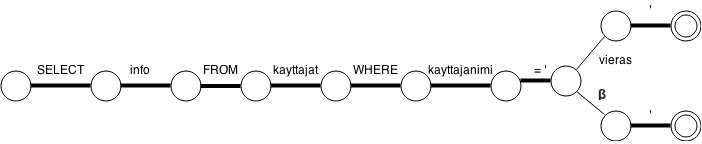
\includegraphics[scale=0.5]{kandi}
		\end{figure}
		
	\subsection{SQLRand}
	SQLRand menetelmä esitellään Boydin ja Keromytisin artikkelissa "SQLrand: Preventing SQL Injection Attacks"\cite{sqlrand}. SQLRandissa on ideana, että normaalit SQL avainsanat kuten "SELECT"\space korvataan satunnaisilla avainsanoilla. Satunnaistaminen tapahtuu lisäämällä alkuperäisen avainsanan perään satunnainen numero. Täten hyökkääjä ei pysty satunnaista numeroa arvaamatta toteuttamaan SQL-injektiota, koska normaalien SQL avainsanojen käyttö aiheuttaa virheilmoituksen. Sovellus tietää virheilmoituksesta että kyseessä oli SQL-injektio.
	\section{Penetraatiotestaus}
	
	 Vaikka sovellusta ohjelmoitaisiin hyvien ohjelmointikäytänteiden mukaisesti, siihen voi silti jäädä tietoturva-aukkoja. Tämän takia sovellusta on jatkuvasti tietoturvatestattava. 
	 
	 Penetraatiotestauksessa yritetään etsiä sovelluksesta tietoturva-aukkoja. Kun penetraatiotestaus on automatisoitua, ohjelmoijan ei tarvitse testata järjestelmäänsä käsin jokaisen muutoksen jälkeen. Automatisoitu testaus ei kuitenkaan ole virheetöntä. Se voi aiheuttaa turhia hälyytyksiä, tai olla hälyyttämättä kun pitäisi hälyyttää \cite{virheita}.  Aiemminkin mainitussa Antunesin ja kumppaneiden tekemässä vertailussa\cite{vertailu} huomattiin, että yli 30\% virheistä oli turhia hälyytyksiä. 
	 
	Musta laatikko -testauksessa testataan sovellusta erilaisia syötteitä vastaan. Tällaiseen testaamiseen ei vaadita pääsyä itse koodiin \cite{testing2}. Tämä on hyödyllistä esimerkiksi sellaisissa tapauksissa, kun osa ohjelman komponenteista on kolmannen osapuolen koodia, eikä siihen päästä käsiksi. Mustalaatikko testauksessa on ongelmana se, että tulos perustuu sovelluksen tulosteesta tehtyyn analyysiin. Tästä syystä kaikkia tietoturva-aukkoja ei välttämättä löydetä, tai jotain turvallista kohtaa koodista voidaan luulla tietoturva-aukoksi. Mustalaatikkotestaukseen löytyy useita valmiita työkaluja, kuten "Acunetix Web Vulnerability Scanner"\space ja sqlmap.
	
	\subsection{Penetraatiotestaus käytännössä}
	 Haixia edottaa artikkelissaan "A database security testing scheme of web application" \cite{testing} seuraavanlaista testausmallia.
	
	Ensiksi etsitään kaikki mahdolliset paikat sovelluksesta, joista käyttäjä voi syöttää dataa. Tämä onnistuu leveyssuuntaista hakua (\textit{engl. Breadth-first search}) käyttämällä. Algoritmi toimii seuraavasti:
	\begin{enumerate}
		\item Alustetaan lista jossa on ainoana jäsenenä etusivun URL. Etusivu merkataan käsittelemättökäks.
		
		\item Käydään listalta läpi kaikki käsittelemättömiksi merkatut sivut. Kunkin sivun kohdalla tehdään seuraavat vaiheet:
		
		- Otetaan talteen kaikki paikat joista käyttäjä voi syöttää dataa.
		
		- Etsitään sivulta kaikki linkit ja lisätään listalle ne jotka eivät vielä ole siellä.
		
		- Merkataan sivu käsitellyksi.
		
		\item Mikäli listalla on käsittelemättömiä linkkejä, palataan vaiheeseen 2.
	\end{enumerate}
	
	Tämän jälkeen luodaan mahdollisimman kattava lista erilaisista hyökkäyksistä. Kaikkiin mahdollisiin paikkoihin joista voi syöttää dataa kokeillaan haitallisia syötteitä. Tietokannan palauttamasta arvosta voidaan päätellä onko injektio onnistunut vai ei. Esimerkiksi jos vastauksen HTTP statuskoodi on 200, kyseessä on haavoittuvuus.
	
	\subsection{Testaussyötteiden luominen}
	Artikkelissa "Automated Testing for SQL Injection Vulnerabilities: An input Mutation Approach"\cite{generation}\space ehdotetaan penetraatiotestauksessa käytettävien syötteiden luomiseen automatisoitua tekniikkaa nimeltään $\mu$SQLi. Tekniikassa on ideana manipuloida kelpaavaa syötettä erilaisilla mutaatio-operaatioilla. Mutaatio-operaatiot jaetaan artikkelin mukaan seuraavalla tavalla kolmeen eri osioon:
	\begin{enumerate}
	\item Käyttäytymistä muuttavat operaatiot
	
	Esimerkiksi operaatiot jotka lisäävät AND tai OR lauseen, tai operaatiot joissa lisätään puolipiste ja kokonaan uusi SQL lause. 
	
	\item Syntax-Repairing Operators
	
	Lisää kyselyyn esimerkiksi sulut, kommenttimerkin tai heittomerkin.
	
	\item Obfuskointi operaatiot
	
	Esimerkiksi muuttaa kyselyssä käytettävää enkoodausta tai muuttaa totuuslauseketta ilman että sen arvo muuttuu.
	\end{enumerate}
	
	Toimivaan syötteeseen voidaa lisätä yksi tai useampi mutaatio-operaatio. Artikkelin mukaan useasti yksittäinen operaatio huomataan, mutta yhdistelmät saattavat silti jäädä huomaamatta. Mutaatioiden tekeminen aloitetaan toimivasta syötteestä, koska sillä vältetään se, että syöte hylättäisiin välittömästi. Lisäksi toimivat syötteet täyttävät todennäköisemmin syötevalidoinnit. 
	
	
	
	\section {Yhteenveto}
	(pahasti kesken)
	
	
	SQL-Injektioilta suojautuminen voidaan jakaa ohjelmointikäytänteisiin, ajonaikaiseen monitorointiin ja testaukseen. Periaatteessa jo hyvät ohjelmointikäytänteet riittävät sovelluksen suojautumiseen SQL-injektiolta. Ei kuitenkaan voida olla varmoja muistetaanko hyviä ohjelmointikäytänteitä aina noudattaa. Tästä syystä on sovellusta tulee penetraatiotestata.
	Penetraatiotestauksessa taas on ongelmana sen luotettavuus. Heikon luotettavuuden takia ei voida koskaan olla varmoja onko sovellus täysin turvallinen. Mitä enemmän menetelmiä käyttää, sitä turvallisempi sovellus on. Menetelmien yhdistely on kuitenkin aikaa vievää. Lisäksi osa menetelmistä tekee sovelluksesta, tai sen tuottamisesta hitaampaa ja monimutkaisempaa. On siis vaikeaa sanoa milloin sovellus on tarpeeksi hyvin suojattu.
	
	SQL-injektio ei kuitenkaan ole ainut tietoturvariski.
	
	
	
	
	% --- References ---
	%
	% bibtex is used to generate the bibliography. The babplain style
	% will generate numeric references (e.g. [1]) appropriate for theoretical
	% computer science. If you need alphanumeric references (e.g [Tur90]), use
	%
	% \bibliographystyle{babalpha-lf}
	%
	% instead.
	
	\bibliographystyle{babplain-lf}
	\bibliography{references-fi}
	
	
	% --- Appendices ---
	
	% uncomment the following
	
	% \newpage
	% \appendix
	% 
	% \section{Esimerkkiliite}
	
\end{document}